\graphicspath{{./figures/}}
\title{}
\date{}
\begin{document}
\begin{frame}
    \titlepage
\end{frame}

{
\setbeamercolor{background canvas}{bg=blue!40!black,fg=blue!10!white}
\setbeamercolor{normal text}{bg=blue!40!black,fg=blue!10!white}
\setbeamercolor{itemize/enumerate body}{fg=white}
\setbeamercolor{itemize/enumerate subbody}{fg=white}
\setbeamercolor{titlelike}{bg=blue!40!black,fg=blue!10!white}
\begin{frame}<1|handout:1>[noframenumbering]{Changelog}
    \begin{itemize}
    \item 22 March 2021 (after lecture): ROP without stack overflow: adjust call gadget into jmp gadget so it is functional
    \item 22 March 2021 (after lecture): add ``if exe addreses fixed'' to ASLR diagrams showing typical locations of executable code loading
    \item 22 March 2021 (after lecture): add diagram illustrating executable staying together before explanation with objdump snippets
    \item 22 March 2021 (after lecture): dependencies between segments (2): correct formatting issue
    \item 22 March 2021 (after lecture): using leak exericses: add explanation slides
    \item 22 March 2021 (after lecture): using leak exericse (2): remove ``in decimal'' from options
    \end{itemize}
\end{frame}
}



\begin{frame}{last time}
    \begin{itemize}
    \item memory protection
        \begin{itemize}
        \item read-only function pointers
        \item write XOR execute
        \end{itemize}
    \item ``gadgets'' in existing code
    \item return-oriented programming
    \end{itemize}
\end{frame}

\begin{frame}{some notes on OBFUSCATE}
    \begin{itemize}
    \item this was an assignment where I most unsure of difficulty callibration
    \vspace{.5cm}
    \item one correct, but unintended solution: 
        \begin{itemize}
        \item the password check used memcmp
        \item not much else used memcmp
        \item could replace memcmp call entirely
        \item probably should've reimplemented that
        \end{itemize}
    \end{itemize}
\end{frame}

\begin{frame}[fragile,label=TTT3]{my TTT3 soln}
\begin{lstlisting}[language=C++,style=smaller]
case 104: 
(PC[0]) ++; /* renamed via find-replace */
/* debug output: */
printf("branch @ PC = %ld\n", PC[0] - CODE[0]);
if (PC[0] - CODE[0] == 2063) { /* found by examining debug output */
    if (!(l___4915[0] + 0)->f___11) {
      PC[0] += *((int *)PC[0]);
    } else {
      PC[0] += 4;
    }
} else {
    if ((l___4915[0] + 0)->f___11) {
      PC[0] += *((int *)PC[0]);
    } else {
      PC[0] += 4;
    }
}    
\end{lstlisting}
\end{frame}


\begin{frame}{on OVER correction}
\end{frame}

\section{ROP con't}

\subsection{example: VTable overwrite}

\begin{frame}{ROP without a stack overflow (1)}
    \begin{itemize}
    \item we can use ROP ideas for non-stack exploits
    \vspace{.5cm}
    \item look for gadget(s) that set {\tt \%rsp}
    \item \ldots based on function argument registers/etc.
    \end{itemize}
\end{frame}

\begin{frame}{ROP without stack overflow (2)}
    \begin{itemize}
    \item example sequence:
        \begin{itemize}
            \item gadget 1: \texttt{push \%rdi; jmp *(\%rdx)}
            \item gadget 2: \texttt{pop \%rsp; ret}
        \end{itemize}
    \item set:
        \begin{itemize}
        \item overwritten function pointer = pointer to gadget 1
        \item arg 1: {\tt \%rdi} = desired stack pointer (pointer to next gadgets)
        \item arg 3: {\tt \%rdx} = pointer to gadget 2
        \end{itemize}
    \end{itemize}
\end{frame}


\usetikzlibrary{arrows.meta,fit,patterns}

\begin{frame}[fragile,label=VTblOver]{VTable overwrite with gadget}
\lstset{language=C++,style=small}
    \begin{tikzpicture}
        \node[anchor=north east] (code) at (1.5, 0) {
\begin{lstlisting}
class Bar {
  char buffer[100];
  Foo *foo;
  int x, y;
  ...
};

void Bar::vulnerable() {
  gets(buffer);
  foo->some_method(x, y);
  // (*foo->vtable[K])(foo, x, y)
  // foo == rdi, x == rsi, y == rdx
}
\end{lstlisting}
};
\tikzset{
    stackBox/.style={very thick},
    onStack/.style={thick},
    useLine/.style={very thick,blue,Latex-},
    useLineRet/.style={red,very thick,-Latex,dashed},
    gadgetBox/.style={blue,thick,text=black,draw,align=left,font=\small},
}
        \begin{visibleenv}<1-2>
\draw[thick,-Latex] (-.25,-4) -- (-.25, -1) node [midway, above, sloped] {increasing addresses};
        \end{visibleenv}
    \draw[stackBox] (0, 0) rectangle (3, -5);
        \draw[onStack,fill=green!20] (0, -1.5) rectangle (3, -5) node[midway] {buffer};
        \draw[onStack,fill=yellow!20] (0, -1) rectangle (3, -1.5) node[midway] {foo};
        \draw[onStack,fill=yellow!20] (0, -0) rectangle (3, -1) node[midway] {x, y};

        \draw[stackBox] (4, 0) rectangle (7, -3);
        \draw[onStack](4, -2.5) rectangle (7, -3) node[midway] {vtable ptr};

        \draw[stackBox] (4, -4) rectangle (7, -6);
        \node[midway,anchor=south] at (5.5, -5) {func. ptrs};
        \draw[fill=blue!30] (4, -5) rectangle (7, -5.5) node[midway] { some\_method };

        \draw[-Latex, very thick,blue] (3, -1.25) -- ++ (.5cm, 0) |- (4, -2.9);
        \draw[-Latex, very thick,blue] (7, -2.75) -- ++ (.5cm, 0) |- (7, -5.9);
        \begin{visibleenv}<2->
            \fill[pattern=north west lines,pattern color=red] (0, -0) rectangle (3, -1.5);
            \draw[-Latex, ultra thick, dashed, red] (3, -1.25) -- ++(.5cm, 0) |- (3, -4.9);
            \draw[fill=white,fill opacity=0.9,draw=red,very thick] (0, -5) rectangle (3, -4.5)
                node[midway] {``vtable'' ptr};
        \end{visibleenv}
        \begin{visibleenv}<3->
            \draw[fill=blue!30,fill opacity=0.9,draw=red,very thick] (0, -2.5) rectangle (3, -2)
                node[midway] {\text{gadget} ptr};
            \draw[-Latex, ultra thick, dashed, red] (0, -4.75) -- ++(-.5cm, 0) |- (0, -3);
            \draw[fill=white,fill opacity=0.9,draw=red,very thick] (0, 0) rectangle (3, -1)
                node[midway] { \textbf{rsi}, \textbf{rdx} values };
            \draw[Latex-, thick,red] (3, -5) -- ++(0cm, -.5cm) node[below] {rdi value};
        \end{visibleenv}
        \begin{visibleenv}<4->
            \node[align=left,thick,draw,anchor=north east,fill=white] (gadget) at (-1, -3) {
                gadget: \\ \texttt{push \%rdx; jmp *(\%rsi)}
            };
            \draw[-Latex,ultra thick, dashed, red] (0, -2.25) -| (gadget.north);
        \end{visibleenv}
    \end{tikzpicture}
\end{frame}




\subsection{definition: JOP}

\begin{frame}{jump-oriented programming}
    \begin{itemize}
        \item seems like \texttt{ret} is the problem?
            \begin{itemize}
            \item solve by protecting rets (e.g. hardware shadow stack)?
            \end{itemize}
        \item problem: don't actually need \texttt{ret}
        \vspace{.5cm}
        \item<2-> just look for gadgets that end in \texttt{call} or \texttt{jmp}
        \item<2-> don't even need to set stack
        \item<2-> harder to find than \texttt{ret}-based gadgets
            \begin{itemize}
            \item but almost always as powerful as ret-based gadgets
            \end{itemize}
    \end{itemize}
\end{frame}


\usetikzlibrary{arrows.meta,matrix}
\begin{frame}[fragile,label=jopdispatch1]{programming JOP}
\begin{tikzpicture}
\node[draw,label={north:``dispatcher'' gadget}]  (code) {
\begin{lstlisting}[language=myasm]
add $8, %rcx
jmp *(%rcx)
\end{lstlisting}
};
\begin{visibleenv}<2->
\matrix[tight matrix,anchor=north west,nodes={font=\small,text width=4cm}] (gadget list) at ([xshift=1cm]code.north east) {
    pointer to gadget1 \\
    pointer to gadget2 \\
    pointer to gadget3 \\
    \ldots \\
};
\path[draw,very thick,Latex-] (gadget list-1-1.east) -- ++(1cm,0cm) node[right] {initial \%rcx};
\path[draw,very thick,Latex-] ([yshift=-.5cm]code.north west) -- ++(-1cm,0cm) node[left] {\%rdx};
\path[draw,very thick,Latex-] ([yshift=-.5cm]code.north west) -- ++(-.5cm, -.5cm) node[draw,very thick,fill=yellow!20,below left] (ptr) {};
\path[draw,very thick,Latex-] (ptr.south) -- ++(0cm, -.5cm) node[below] {\%rdi};
\path[draw,thick,dotted,-Latex] ([xshift=-.1cm]gadget list-1-1.north west) -- ++(0cm, -1cm);
\end{visibleenv}
\begin{visibleenv}<3->
\node[draw,label={north:template for other gadgets}] (code 2) at ([xshift=1cm,yshift=-3cm]code.south east) {
\begin{lstlisting}[language=myasm]
...
jmp *%rdx
\end{lstlisting}
---\textit{ OR }---
\begin{lstlisting}[language=myasm]
...
jmp *(%rdi)
\end{lstlisting}
};
\end{visibleenv}
\end{tikzpicture}
\begin{itemize}
\item<4-> setup: find a way to set \%rdx, \%rdi, \%rcx appropriately
\item<5-> note: can choose different registers, dispatcher design
\end{itemize}
\end{frame}

\begin{frame}[fragile,label=jopdispatch2]{dispatcher gadgets?}
\begin{lstlisting}[language={},style=smaller]
/* from libc on my desktop: */
adc esi, edi ; jmp qword ptr [rsi + 0xf]
add al, ch ; jmp qword ptr [rax - 0xe]

/* from firefox on my desktop: */
add eax, ebp ; jmp qword ptr [rax]
add edi, -8 ; mov rax, qword ptr [rdi] ; jmp qword ptr [rax + 0x68]
sub esi, dword ptr [rsi] ; jmp qword ptr [rsi - 0x7d]
\end{lstlisting}
\begin{itemize}
\item adc (add with carry) --- Intel syntax: destination first
\end{itemize}
\end{frame}


\subsection{exercise: using function pointer overwrite}
\begin{frame}[fragile,label=useFPtrOverwrite1]{using function pointer overwrite (1)}
\begin{lstlisting}[language=C,style=script]
struct Example {
    char input[1000];
    void (*process_function)(Example *, long, char *);
};
void vulnerable(struct Example *e) {
    long index;
    char name[1000];
    gets(e->input); /* can overwrite process_function */
    scanf("%ld,%s", &index, &name[0]); /* expects <decimal number>,<string> */
    (e->process_function)(e /* rdi */, index /* rsi */, name /* rdx */);
}
\end{lstlisting}
\begin{itemize}
\item if we overwrite process\_function's address with the address of the gadget
    \texttt{mov \%rsi, \%rsp; ret}, then the beginning of the input
    should contain\ldots \\
    \begin{itemize}
    \item A. the shellcode to run
    \item B. an ROP chain to run
    \item C. the address of shellcode (or existing function) in decimal
    \item D. the address of the ROP chain to run written out in decimal
    \item E. the address of a RET instruction written out in decimal
    \end{itemize}
\end{itemize}
\end{frame}

\iftoggle{heldback}{\excludecomment{soln}}{\includecomment{soln}}
\begin{soln}
\begin{frame}[fragile,label=useFPtrOverwrite1Explain]{explanation}
\begin{lstlisting}[language=C++,style=script]
gets(e->input); /* can overwrite process_function */
scanf("%ld,%s", &index, &name[0]); /* expects <decimal number>,<string> */
(e->process_function)(e /* rdi */, index /* rsi */, name /* rdx */);
\end{lstlisting}
\texttt{"1234,FOO......."} + addr of \texttt{mov \%rsi, \%rsp, ret}
\begin{itemize}
\item arguments setup registers for gadget:
\begin{itemize}
    \item \%rdi (irrelevant) is "1234,FOO..." (copy in e)
    \item \%rsi is 1234 (from scanf)
    \item \%rdx (irrelevant) is "FOO..." (pointer to name)
\end{itemize}
\item mov in gadget: \%rsi (1234) becomes \%rsp
\item ret in gadget: read pointer at 1234, set \%rsp to 1234 + 8
    \begin{itemize}
    \item jump to next gadget (whose address should be stored at 1234)
    \item if that gadget returns, will read new return address from 1238
    \end{itemize}
\end{itemize}
\end{frame}
\end{soln}

\begin{frame}[fragile,label=useFPtrOverwrite2]{using function pointer overwrite (2)}
\begin{lstlisting}[language=C,style=script]
struct Example {
    char input[1000];
    void (*process_function)(Example *, long, char *);
};
void vulnerable(struct Example *e) {
    long index;
    char name[1000];
    gets(e->input); /* can overwrite process_function */
    scanf("%ld,%s", &index, &name[0]); /* expects <decimal number>,<string> */
    (e->process_function)(e /* rdi */, index /* rsi */, name /* rdx */);
}
\end{lstlisting}
\begin{itemize}
\item if we overwrite process\_function's address with the address of the gadget
    \texttt{push \%rdx; jmp *(\%rdi)}, then the beginning of the input should contain\ldots \\
    \begin{itemize}
    \item A. the shellcode to run
    \item B. an ROP chain to run
    \item C. the address of shellcode (or existing function) 
    \item D. the address of the ROP chain 
    \item E. the address of a RET instruction
    \end{itemize}
\end{itemize}
\end{frame}

\begin{soln}
\begin{frame}[fragile,label=useFPtrOverwrite1Explain]{explanation (one option)}
\begin{lstlisting}[language=C++,style=script]
gets(e->input); /* can overwrite process_function */
scanf("%ld,%s", &index, &name[0]); /* expects <decimal number>,<string> */
(e->process_function)(e /* rdi */, index /* rsi */, name /* rdx */);
\end{lstlisting}
\texttt{"FOOBARBAZ......."} + addr of \texttt{push \%rdx; jmp *(\%rdi)}
\begin{itemize}
\item arguments setup registers for gadget:
\begin{itemize}
    \item \%rdi is "FOOBARBAZ...." (copy in e)
    \item \%rsi (irrelevant) is uninitialized? (scanf failed)
    \item \%rdx (irrelevant) is uninitialized? (scanf failed)
\end{itemize}
\item push in gadget: top of stack becomes copy of uninit. value 
\item jmp in gadget
    \begin{itemize}
    \item interpret ``FOOBARBA'' as 8-byte address
    \item jump to that address
    \end{itemize}
\end{itemize}
\end{frame}

\begin{frame}[fragile,label=useFPtrOverwrite2Explain]{explanation (unlikely alternative?)}
\begin{lstlisting}[language=C++,style=script]
gets(e->input); /* can overwrite process_function */
scanf("%ld,%s", &index, &name[0]); /* expects <decimal number>,<string> */
(e->process_function)(e /* rdi */, index /* rsi */, name /* rdx */);
\end{lstlisting}
\texttt{"1234567890,FOO......."} + addr of \texttt{push \%rdx; jmp *(\%rdi)}
\begin{itemize}
\item arguments setup registers for gadget:
\begin{itemize}
    \item \%rdi is address of string "12345678,FOO..." (copy in e)
    \item \%rsi is 12345678
    \item \%rdx is address of string "FOO..." (copy in name)
\end{itemize}
\item push in gadget: top of stack becomes address of "FOO..."
\item jmp in gadget
    \begin{itemize}
    \item interpret \textit{ASCII encoding of ``12345678''} (???) as 8-byte address
    \item jump to that address
    \end{itemize}
\end{itemize}
\end{frame}
\end{soln}


\subsection{just get rid of rets?}
\begin{frame}{can we get rid of gadgets? (1)}
    \begin{itemize}
    \item Onarlioglu et al, ``G-Free: Defeating Return-Oriented Programming through Gadget-Less Binaries'' (2010)
    \item two parts:
        \begin{itemize}
        \item get rid of unintended jmp, ret instructions
        \item add stack canary-like checks to jmp, ret instructions
        \end{itemize}
    \item hope: no \textit{useful} gadgets b/c of canary-like checks
        \begin{itemize}
        \item all gadgets should be useless without a secret value?
        \item still vulnerable to information leaks
        \end{itemize}
    \item overhead is not low:
        \begin{itemize}
        \item 20--30\% (!) space overhead
        \item 0--6\% time overhead
        \end{itemize}
    \end{itemize}
\end{frame}

\begin{frame}{no unintended jmp/ret (1)}
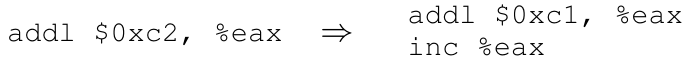
\includegraphics[width=10cm]{../mitigate/gfree1}
\begin{itemize}
\item \texttt{addl \$0xc2, \%eax}: \texttt{05 \myemph<2>{c2 00 00} 00}
\item problem: \texttt{\myemph<2>{c2 00 00}}: variant of ret instruction
\item paper's proposed fix: change the constant
\end{itemize}
\end{frame}

\begin{frame}{no unintended jmp/ret (2)}
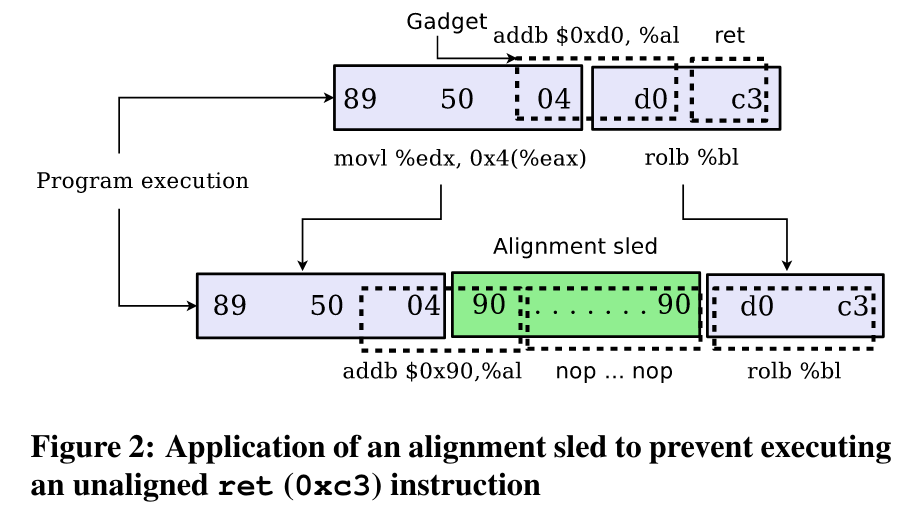
\includegraphics[width=10cm]{../mitigate/gfree2}
\end{frame}


\section{ASLR}
\subsection{what it is}

\begin{frame}{address space layout randomization (ASLR)}
    \begin{itemize}
    \item assume: addresses don't leak
    \item choose \myemph{random} addresses each time
        \begin{itemize}
        \item for \myemph{everything}, not just the stack
        \end{itemize}
    \item \myemph{enough possibilities} that attacker won't ``get lucky''
    \item should prevent exploits --- can't write GOT/shellcode location
    \end{itemize}
\end{frame}



\subsection{how much entropy}
\usetikzlibrary{calc,positioning,patterns,shapes.callouts}

\begin{frame}{Linux stack randomization (x86-64)}
\begin{itemize}
    \item 1. choose random number between \texttt{0} and \tikzmark{range}\myemph<2>{\texttt{0x3F FFFF}}
    \item 2. stack starts at \texttt{0x7FFF FFFF FFFF} - \textit{random number} $\times$ \texttt{0x1000}
        \begin{itemize}
        \item randomization disabled? \textit{random number} $= 0$
        \end{itemize}
\end{itemize}
\begin{tikzpicture}[overlay,remember picture]
\node[my callout=range] at ([yshift=-1cm]current page.center) {
    16 GB range!
};
\end{tikzpicture}
\end{frame}

\begin{frame}<1>[fragile,label=aslr64]{program memory (x86-64 Linux; ASLR)}
\begin{tikzpicture}[remember picture]
\tikzset{
    mylabel/.style={font=\ttfamily,align=center,append after command={([xshift=.1cm]\tikzlastnode.west) edge[ultra thick] ++(-.2cm,0cm)}},
    mybox/.style={draw,rectangle,minimum width=7cm,fill=white},
    myhigh/.style={draw,rectangle,line width=1mm, draw=blue!80!black,opacity=.3},
}
\node[mybox,minimum height=.5cm,inner ysep=0mm,pattern=north west lines,pattern color=black!50!white] (kernel) {Used by OS};
\begin{pgfonlayer}{bg}
    \node[right=1mm of kernel.north east,mylabel] (topLabel) {0xFFFF FFFF FFFF FFFF};
    \node[right=1mm of kernel.south east,mylabel] {0xFFFF 8000 0000 0000};
\end{pgfonlayer}
\node[mybox, minimum height=.5cm, below=.45cm of kernel] (stack) {Stack};
\begin{pgfonlayer}{bg}
    \node[right=1mm of stack.north east,mylabel] {\myemph<1>{$\pm$ 0x004 0000 0000}};
\end{pgfonlayer}
\node[mybox, minimum height=.5cm, below=0.5cm of stack] (heapB) {Dynamic/Non-fixed exe/Libraries (mmap)};
\begin{pgfonlayer}{bg}
    \node[right=1mm of heapB.north east,mylabel] (heapBLabel) {\myemph<1>{$\pm$ 0x100 0000 0000}};
    \node[below=0mm of heapBLabel,font=\small,inner sep=0mm] {(filled from top with ASLR)};
\end{pgfonlayer}
%\begin{pgfonlayer}{bg}
%    \node[right=1mm of heapB.south east,mylabel] (heapBLabel) {0x0000 2baa aaaa b000 \\ $\pm$ 0x100 0000 0000\*};
%\end{pgfonlayer}
\node[mybox, minimum height=.5cm, below=0.5cm of heapB] (heap) {Heap (brk/sbrk)};
\begin{pgfonlayer}{bg}
\node[right=1mm of heap.south east,mylabel] (heapBLabel) {\myemph<1>{$\pm$ 0x200 0000}};
\end{pgfonlayer}
\node[mybox, minimum height=.5cm, below=0.2mm of heap] (data) {Writable data if fixed exe addresses};
\begin{pgfonlayer}{bg}
\node[right=1mm of data.south east,mylabel] (bottomLabel) {\myemph<2-3>{0x0000 0000 0060 0000}*};
\node[below=0mm of bottomLabel,font=\small,inner sep=0mm] {(constants + 2MB alignment)};
\end{pgfonlayer}
\node[mybox, minimum height=.5cm, below=0.6cm of data] (sdata) {Code + Constants if fixed exe addresses};
\begin{pgfonlayer}{bg}
\node[right=1mm of sdata.south east,mylabel] (sbottomLabel) {\myemph<2-3>{0x0000 0000 0040 0000}};
\end{pgfonlayer}
\coordinate (memBottom) at ($(sdata.south east) + (0mm, -2mm)$);
\begin{pgfonlayer}{bg}
\draw[pattern=north west lines, pattern color=black!40!white] (kernel.north west) rectangle (memBottom);
\end{pgfonlayer}

\begin{visibleenv}<3>
    \begin{scope}[overlay]
    \node[draw=red,ultra thick,fill=white,anchor=center,
          inner sep=.5cm,font=\Large] at (current page.center) {
        why are these addresses fixed?
    }; 
    \end{scope}
\end{visibleenv}

\end{tikzpicture}
\end{frame}

\begin{frame}{program memory (x86-32 Linux; ASLR)}
\begin{tikzpicture}
\tikzset{
    mylabel/.style={font=\ttfamily,align=center,append after command={([xshift=.1cm]\tikzlastnode.west) edge[ultra thick] ++(-.2cm,0cm)}},
    mybox/.style={draw,rectangle,minimum width=7cm,fill=white},
    myhigh/.style={draw,rectangle,line width=1mm, draw=blue!80!black,opacity=.3},
}
\node[mybox,minimum height=.5cm,inner ysep=0mm,pattern=north west lines,pattern color=black!50!white] (kernel) {Used by OS};
\begin{pgfonlayer}{bg}
    \node[right=1mm of kernel.north east,mylabel] (topLabel) {0xFFFF FFFF};
    \node[right=1mm of kernel.south east,mylabel] {0xC000 0000};
\end{pgfonlayer}
\node[mybox, minimum height=.5cm, below=.5cm of kernel] (stack) {Stack};
\begin{pgfonlayer}{bg}
    \node[right=1mm of stack.north east,mylabel] {\myemph{$\pm$ 0x080 0000} (default)};
\end{pgfonlayer}
\node[mybox, minimum height=.5cm, below=0.5cm of stack] (heapB) {Dynamic/Libraries (mmap)};
\begin{pgfonlayer}{bg}
    \node[right=1mm of heapB.north east,mylabel] (heapBLabel) {\myemph{$\pm$ 0x008 0000} (default)};
\end{pgfonlayer}
%\begin{pgfonlayer}{bg}
%    \node[right=1mm of heapB.south east,mylabel] (heapBLabel) {0x0000 2baa aaaa b000 \\ $\pm$ 0x100 0000 0000\*};
%\end{pgfonlayer}
\node[mybox, minimum height=.5cm, below=0.5cm of heapB] (heap) {Heap (brk/sbrk)};
\begin{pgfonlayer}{bg}
\node[right=1mm of heap.south east,mylabel] (heapBLabel) {\myemph{$\pm$ 0x200 0000}};
\end{pgfonlayer}
\node[mybox, minimum height=.5cm, below=0.2mm of heap] (data) {Writable data};
\begin{pgfonlayer}{bg}
%\node[right=1mm of data.south east,mylabel] (bottomLabel) {0x0804 0000};
\end{pgfonlayer}
\node[mybox, minimum height=.5cm, below=0.6cm of data] (sdata) {Code + Constants if fixed exe addresses};
\begin{pgfonlayer}{bg}
\node[right=1mm of sdata.south east,mylabel] (bottomLabel) {0x0804 8000};
\end{pgfonlayer}
\coordinate (memBottom) at ($(sdata.south east) + (0mm, -2mm)$);
\begin{pgfonlayer}{bg}
\draw[pattern=north west lines, pattern color=black!40!white] (kernel.north west) rectangle (memBottom);
\end{pgfonlayer}
\end{tikzpicture}
\end{frame}

\begin{frame}{how much guessing?}
    \begin{itemize}
    \item gaps change by multiples of page (4K)
        \begin{itemize}
        \item lower 12 bits are \myemph{fixed}
        \end{itemize}
    \item 64-bit: \myemph{huge} ranges --- need millions of guesses
        \begin{itemize}
        \item about \myemph{30 randomized bits} in addresses
        \end{itemize}
    \item 32-bit: \myemph{smaller} ranges --- hundreds of guesses
        \begin{itemize}
        \item only about \myemph{8 randomized bits} in addresses
        \item why? only 4 GB to work with!
        \item can be configured higher --- but larger gaps
        \end{itemize}
    \end{itemize}
\end{frame}

\begin{frame}{why do we get multiple guesses?}
    \begin{itemize}
    \item why do we get multiple guesses?
    \vspace{.5cm}
    \item wrong guess might not crash
    \item wrong guess might not crash whole application
        \begin{itemize}
        \item e.g. server that uses multiple processes
        \end{itemize}
    \item local programs we can repeatedly run
    \item servers that are automatically restarted
    \end{itemize}
\end{frame}


\subsection{kept together: danger of leaks}

\begin{frame}[fragile,label=betweenSegments1]{dependencies between segments (1)}
\begin{lstlisting}[language={},style=smaller]
$ objdump -x foo.exe
...
LOAD off    0x0000000000000000 vaddr 0x0000000000000000 paddr 0x0000000000000000 align 2**12
     filesz 0x0000000000000620 memsz 0x0000000000000620 flags r--
LOAD off    0x0000000000001000 vaddr 0x0000000000001000 paddr 0x0000000000001000 align 2**12
     filesz 0x0000000000000205 memsz 0x0000000000000205 flags r-x
LOAD off    0x0000000000002000 vaddr 0x0000000000002000 paddr 0x0000000000002000 align 2**12
     filesz 0x0000000000000150 memsz 0x0000000000000150 flags r--
LOAD off    0x0000000000002db8 vaddr 0x0000000000003db8 paddr 0x0000000000003db8 align 2**12
     filesz 0x000000000000025c memsz 0x0000000000000260 flags rw-
\end{lstlisting}
\begin{itemize}
\item 4 seperately loaded segments: can we choose random addresses for each?
\end{itemize}
\end{frame}

\begin{frame}[fragile,label=betweenSegments2]{dependencies between segments (2)}
\begin{lstlisting}[language={},style=smaller,moredelim={**[is][\btHL<1->]{~2~}{~end~}}]
0000000000001050 <__printf_chk@plt>:
    1050:       f3 0f 1e fa             endbr64 
    1054:       f2 ff 25 75 2f 00 00    bnd jmpq *~2~0x2f75(%rip)        # 3fd0~end~ <__printf_chk@GLIBC_2.3.4>
    105b:       0f 1f 44 00 00          nopl   0x0(%rax,%rax,1)
\end{lstlisting}
\begin{itemize}
\item dependency from 2nd LOAD (0x1000-0x1205) to 4th LOAD (0x3db8-0x4018)
\item uses relative addressing rather than linker filling in address
\end{itemize}
\end{frame}

\begin{frame}[fragile,label=betweenSegments3]{dependencies between segments (3)}
\begin{lstlisting}[language={},style=smaller,moredelim={**[is][\btHL<1->]{~2~}{~end~}}]
0000000000001060 <main>:
    1060:       f3 0f 1e fa             endbr64 
    1064:       50                      push   %rax
    1065:       8b 15 a5 2f 00 00       mov    0x2fa5(%rip),%edx        # 4010 <global>
    106b:       48 8d 35 92 0f 00 00    lea    ~2~0xf92(%rip)~end~,%rsi        # 2004 <_IO_stdin_used+0x4>
    1072:       31 c0                   xor    %eax,%eax
    1074:       bf 01 00 00 00          mov    $0x1,%edi
    1079:       e8 d2 ff ff ff          callq  1050 <__printf_chk@plt>
\end{lstlisting}
\begin{itemize}
\item dependency from 2nd LOAD (0x1000-0x1205) to 3rd LOAD (0x2000-0x2150)
\item uses relative addressing rather than linker filling in address
\end{itemize}
\end{frame}

\begin{frame}[fragile,label=whyRipRelative]{why is this done?}
\begin{itemize}
\item Linux made a choice: \\
no editing code when loading programs, libraries\
\vspace{.5cm}
\item allows same code to be loaded in multiple processes
\end{itemize}
\end{frame}

\begin{frame}[fragile,label=noGuessing]{danger of leaking pointers}
    \begin{itemize}
        \item any stack pointer? know everything on the stack!
        \item any pointer within executable? know everything in the executable!
        \item any pointer to a particular library? know everything in library!
    \end{itemize}
\end{frame}



\subsection{exercise: using a leak}
\begin{frame}[fragile,label=useLeak1]{exericse: using a leak (1)}
\begin{lstlisting}[language=C++,style=small]
class Foo {
    virtual const char *bar() { ... }
};
...
Foo *f = new Foo;
printf("%s\n", f);
\end{lstlisting}
\begin{itemize}
\item Part 1: What address is most likely leaked by the above?
    \begin{itemize}
    \item A. the location of the Foo object allocated on the heap
    \item B. the location of the first entry in Foo's VTable"
    \item C. the location of the first instruction of Foo::Foo() (Foo's compiler-generated constructor)"
    \item D. the location of the stack pointer
    \end{itemize}
\end{itemize}
\end{frame}


\begin{frame}[fragile,label=useLeak2]{exercise: using a leak (2)}
\begin{lstlisting}[language=C++,style=script]
class Foo {
    virtual const char *bar() { ... }
};
...
Foo *f = new Foo;
char *p = new char[1024];
printf("%s\n", f);
\end{lstlisting}
\begin{itemize}
\item if leaked value was 0x822003 and in a debugger (with \textbf{different randomization}):
    \begin{itemize}
    \item stack pointer was 0x7ffff000
    \item Foo::bar's address was 0x400000
    \item f's address was 0x900000
    \item f's Vtable's address was 0x403000
    \item a ``gadget'' address from the main executable was 0x401034
    \item a ``gadget'' address from the C library was 0x2aaaa40034
    \item p's address was 0x901000
    \end{itemize}
\item which of the above can I compute based on the leak?
\end{itemize}
\end{frame}

\usetikzlibrary{arrows.meta,decorations.pathreplacing,decorations.pathmorphing}
\begin{frame}<1>[fragile,label=aslrTogether]{exes, libraries stay together}
\begin{tikzpicture}[remember picture]
\draw[thick,decorate,decoration={zigzag}] (0, 0) -- (6, 0);
\draw[thick] (0, 0) -- (0, -7);
\draw[thick] (6, 0) -- (6, -7);
\draw[thick,decorate,decoration={zigzag}] (0, -7) -- (6, -7);
\draw[thick,fill=yellow!10] (0, -1) rectangle ++(6, -0.8) node[midway] {foo.exe globals};
\draw[thick,fill=yellow!10] (0, -2) rectangle ++(6, -1.3) node[midway] {foo.exe code};
\draw[thick,fill=yellow!10] (0, -3.5) rectangle ++(6, -0.9) node[midway,align=center] {foo.exe constants \\ (likely has VTables)};
\draw[very thick,Latex-] (6, -4.4) -- ++ (1cm, 0cm) node[right] {this address can be randomized};
\draw[very thick,decorate,decoration={brace,mirror}] (6.1, -4.4) -- ++ (0cm, 3.4) node[midway,right,align=left] {
    must stay together \\
    code uses offset(\%rip) \\
    to access globals, constants
};
\end{tikzpicture}
\end{frame}



\section{backup slides}
\begin{frame}{backup slides}
\end{frame}


\begin{frame}[fragile,label=reloc]{recall: relocation}
\lstset{
    language=myasm,
    style=small,
    moredelim={**[is][\btHL<1>]{~1~}{~end~}},
    moredelim={**[is][\btHL<2>]{~2~}{~end~}},
}
\begin{lstlisting}
.data
string: .asciz "Hello, World!"
.text
main:
    movq $~1~string~end~, %rdi /* NOT PC/RIP-relative mov */
\end{lstlisting}
    generates: (\texttt{objdump --disassemble --reloc})
\lstset{
    language={},
    style=small,
    moredelim={**[is][\btHL<1>]{~1~}{~end~}},
    moredelim={**[is][\btHL<2>]{~2~}{~end~}},
}
\begin{lstlisting}
   0:   48 c7 c7 00 00 00 00    mov    $0x0,%rdi
                        ~1~3: R_X86_64_32S .data~end~
\end{lstlisting}
    \begin{itemize}
        \item \myemph{relocation record} says how to fix \texttt{0x0} in \texttt{mov}
            \begin{itemize}
                \item 3: location in machine code
                \item \texttt{R\_X86\_64\_32S}: 32-bit signed integer
                \item \texttt{.data}: address to insert
            \end{itemize}
    \end{itemize}
\end{frame}




% FIXME: weird machines

\subsection{weird machines}
\begin{frame}{programs as weird machines}
    \begin{itemize}
    \item ROP, format strings: mini machine language
    \item set of instructions including:
        \begin{itemize}
        \item reading/writing values from memory
        \item flow control
        \item make system calls (requests to operating system)
        \end{itemize}
    \item can be viewed as virtual machine with unusual instruction set
    \vspace{.5cm}
    \item can be analyzed using DMT2 techniques
        \begin{itemize}
        \item what can it compute?
        \end{itemize}
    \end{itemize}
\end{frame}


\subsection{finding gadgets, generally}

\begin{frame}{finding gadgets}
    \begin{itemize}
        \item find code segments of exectuable/library
        \item look for opcodes of arbitrary jumps:
            \begin{itemize}
            \item \texttt{ret}
            \item \texttt{jmp *register}
            \item \texttt{jmp *(register)}
            \item \texttt{call *register}
            \item \texttt{call *(register)}
        \end{itemize}
        \item disassemble starting a few bytes before
            \begin{itemize}
            \item invalid instruction? jump before ret? etc. --- discard
            \end{itemize}
        \item sort list
        \vspace{.5cm}
    \item \myemph{automatable}
    \end{itemize}
\end{frame}

\begin{frame}[fragile,label=ROPgadgetEx1]{ROPgadget}
    \begin{itemize}
    \item ROPgadget: tool that does this
    \end{itemize}
\begin{lstlisting}[language={},style=small]
$ ROPgadget --binary /bin/ls
....
0x000000000000f09d : xor r8d, r8d ; cmp rcx, rsi ; jb 0xf0b9 ; jmp 0xf0e6
0x0000000000012a22 : xor r8d, r8d ; jmp 0x11fee
0x0000000000013d86 : xor r8d, r8d ; jmp 0x137a8
0x000000000001421a : xor r8d, r8d ; jmp 0x141b0
0x0000000000006aa1 : xor r8d, r8d ; jmp 0x69d5
0x00000000000099f0 : xor r8d, r8d ; jmp 0x931d
0x000000000000e6d0 : xor r8d, r8d ; mov rax, r8 ; ret
0x00000000000127a7 : xor r8d, r8d ; xor esi, esi ; jmp 0x11fee
0x000000000000e640 : xor r8d, r8d ; xor esi, esi ; jmp 0xe66a
0x000000000001435d : xor r9d, r9d ; jmp 0x141b0
0x0000000000008a03 : xor r9d, r9d ; xor r12d, r12d ; jmp 0x873c
0x0000000000014217 : xor r9d, r9d ; xor r8d, r8d ; jmp 0x141b0

Unique gadgets found: 6472
\end{lstlisting}
\end{frame}

\begin{frame}{selected ROP gadget options}
    \begin{itemize}
    \item {\tt --offset X}: set start location for binray/library
    \item {\tt --badbytes XYZ}: ignores gadgets whose addresses contain cerain bytes
        \begin{itemize}
        \item to handle restrictions on input --- e.g no newline
        \item similar to writing shellcode without specific bytes
        \end{itemize}
    \end{itemize}
\end{frame}


% FIXME: demo

\subsection{reusable sequence}

\begin{frame}{common, reusable ROP sequences}
    \begin{itemize}
        \item most common idea: run a shell (command prompt)
            \begin{itemize}
            \item same thing `shellcode is named after'
            \item \texttt{ROPchain --binary example --ropchain} tries to do this
            \end{itemize}
        \item another possibilities: make memory executable + jump
            \begin{itemize}
            \item make `normal' shellcode work
            \end{itemize}
        \item probably more ideas
        \vspace{.5cm}
        \item if finding one of these in popular library\ldots
        \item can reuse across a lot of applications
    \end{itemize}
\end{frame}

\begin{frame}[fragile,label=ropchainex1]{ROPgadget --ropchain (works)}
\begin{lstlisting}[language={},style=script]
ROPgadget --binary /lib/x86_64-linux-gnu/libc.so.6 \
             --offset 0x10000000 --ropchain
...
        #!/usr/bin/env python
        # execve generated by ROPgadget

        from struct import pack

        # Padding goes here
        p = b''
        p += pack('<Q', 0x00000000101056fd) # pop rdx ; pop rcx ; pop rbx ; ret
        p += pack('<Q', 0x00000000101eb1a0) # @ .data
        p += pack('<Q', 0x4141414141414141) # padding
        p += pack('<Q', 0x4141414141414141) # padding
        p += pack('<Q', 0x000000001004a550) # pop rax ; ret
        p += '/bin//sh'
        p += pack('<Q', 0x00000000100374b0) # mov qword ptr [rdx], rax ; ret
...
\end{lstlisting}
\end{frame}

\begin{frame}[fragile,label=ropchainex]{ROPgadget --ropchain (does not work?)}
\begin{lstlisting}[language={},style=script]
ROPgadget --binary /bin/ls --ropchain
...
ROP chain generation
===========================================================

- Step 1 -- Write-what-where gadgets

        [+] Gadget found: 0x7694 mov byte ptr [rax], 0xa ; pop rbx ; pop rbp ; pop r12 ; ret
        [-] Can't find the 'pop rax' gadget. Try with another 'mov [reg], reg'

        [-] Can't find the 'mov qword ptr [r64], r64' gadget
...
\end{lstlisting}
\end{frame}


\end{document}
